\usetikzlibrary{calc,arrows.meta,patterns,angles,quotes}
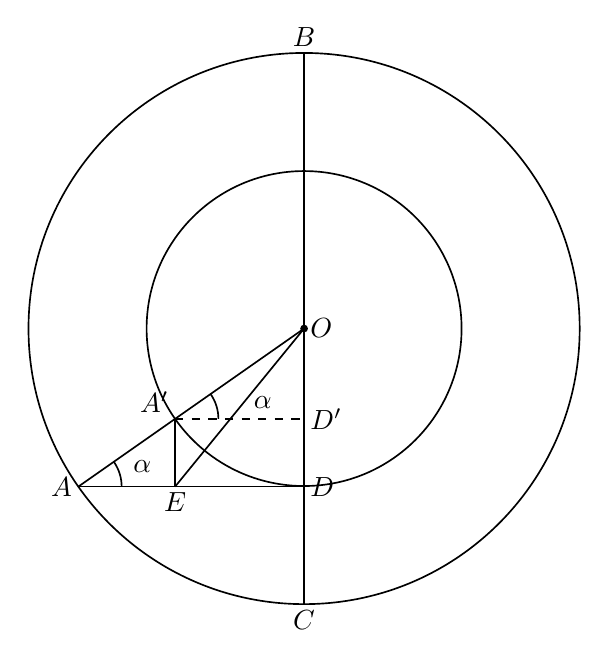
\begin{tikzpicture}[x=1cm,y=1cm,line width=.6pt,font=\normalsize,>=Stealth]
\coordinate (O) at (0.0000000000,0.0000000000);
\coordinate (B) at (0.0000000000,3.5000000000);
\coordinate (C) at (0.0000000000,-3.5000000000);
\coordinate (A) at (-2.8670321550,-2.0075175272);
\coordinate (D) at (0.0000000000,-2.0075175272);
\coordinate (Ap) at (-1.6383040886,-1.1471528727);
\coordinate (E) at (-1.6383040886,-2.0075175272);
\coordinate (Dp) at (0.0000000000,-1.1471528727);
\draw (O) circle[radius=3.5000000000cm];
\draw (O) circle[radius=2.0000000000cm];
\draw (B)--(C);
\draw (A)--(D);
\draw (Ap)--(E);
\draw (O)--(A);
\draw (E)--(O);
\draw[dashed] (Ap)--(Dp);
\draw (-2.3170321550,-2.0075175272) arc[start angle=0.0000000000,end angle=35.0000000000,radius=0.5500000000cm];
\draw (-1.0883040886,-1.1471528727) arc[start angle=0.0000000000,end angle=35.0000000000,radius=0.5500000000cm];
\node[above=2pt,inner sep=0pt] at (B) {$B$};
\node[below=2pt,inner sep=0pt] at (C) {$C$};
\node[right=2pt,inner sep=0pt] at (O) {$O$};
\node[left=2pt,inner sep=0pt] at (A) {$A$};
\node[right=2pt,inner sep=0pt] at (D) {$D$};
\node[below=2pt,inner sep=0pt] at (E) {$E$};
\node[above left=2pt,inner sep=0pt] at (Ap) {$A'$};\node[right=2pt,inner sep=0pt] at (Dp) {$D'$};
\node at (-2.0563727469,-1.7519175977) {$\alpha$};
\node at (-0.5231924906,-0.9369776586) {$\alpha$};

% Explicit named circle-center points, painted after all region fills.
\fill (O) circle[radius=1.4pt];
\end{tikzpicture}
